\documentclass[tikz]{standalone}
\usepackage{pgfplots}
\usepackage{xcolor}
\usetikzlibrary{calc}
\definecolor{mycolor}{HTML}{6d9eeb}
\pgfplotsset{compat=1.18}

\begin{document}
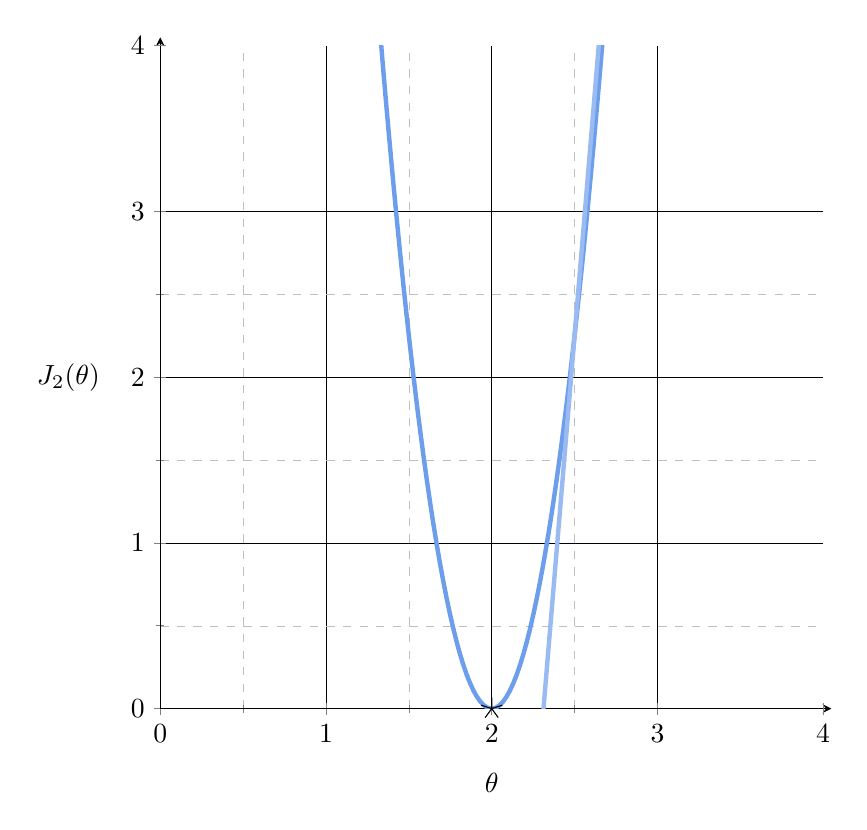
\begin{tikzpicture}
  \begin{axis}[
    axis lines=left,
    x axis line style={->,>=stealth, shorten >=-3pt},
    y axis line style={->,>=stealth, shorten >=-3pt},
    xlabel={\(\theta\)},
    ylabel={\(J_2(\theta)\)},
    ylabel style={rotate=-90},
    xmin=0, xmax=4,
    ymin=0, ymax=4,
    xtick={0,1,...,3},
    ytick={0,1,...,3},
    extra x ticks={4},
    extra x tick style={grid=none},
    extra y ticks={4},
    extra y tick style={grid=none},
    minor x tick num=1,
    minor y tick num=1,
    grid=both,
    major grid style={line width=0.2pt,draw=black},
    minor grid style={line width=0.1pt,draw=gray!50,dashed},
    width=10cm,
    height=10cm,
  ]
    % Plot the single error term (without 1/3): (3θ-6)^2
    \addplot[domain=0:4, samples=200, ultra thick, color=mycolor]
      {(3*x-6)^2};

    % Tangent line at θ=2.5: slope 12 → y = 12(x-2.5)+J(2.5)
    % J(θ) = (3θ-6)^2, so J(2.5) = (7.5-6)^2 = 2.25 and J'(θ)=2(3θ-6)*3 → J'(2.5)=12
    \addplot[domain=0:4, samples=2, ultra thick, color=mycolor!70]
      {12*(x-2.5)+2.25};

    % Mark the minimum at θ=2
    \addplot[only marks, mark=star, mark options={scale=2, fill=red}] 
    coordinates {(2,0)};
  \end{axis}
\end{tikzpicture}
\end{document}


